\section{Publications}
\label{sec:pubs}

This section gives pointers to recent publications about the three CV tasks:  {\em visual saliency, object/scene identification and image classification}.

\subsection{Saliency}

The research question is how can the CV system determine automatically the most visually {\em salient} region(s) in an image? Saliency refers to features like distinctiveness (standing out), catching the focus of attention, characteristic. Usually a salient object of interest is sought to be separated from the background. Automatic measures of saliency are based on measurable properties of the object,

In \cite{LiuCVPR2007} the salient object detection is formulated as image segmentation problem. The object is separated from the background on the basis of several features including multi-scale contrast, center-surround histogram and color spatial distribution for the object description on several levels- locally, regionally and globally. The multi-scale contrast is the local feature, the center-surround histogram is the regional feature and the color spatial histogram- the global. These features are illustrated on Figure \ref{fig:sal_feat_liu07}.
\begin{figure}[H]
\begin{center}
\includegraphics[width=0.95\textwidth]{fig/SalientFeatures_Liu2007}
\end{center}
\caption{Examples of salient features. From left to right: input image, multi-scale contrast, center-surround histogram, color spatial distribution and binary salient mask by CRF.}
\label{fig:sal_feat_liu07}
\end{figure}
A conditional Random Field is trained on these features. 
For the purposes of this research the authors have compiled a large-scale database, MSRA (\cite{msra_db}), presented in section \ref{subsec:msra}. The database is publicly available, while the software is not. The proposed methods compared to two other algorithms ``FG" (fuzzy growing) and ``SM" (salient model as computed by the SalientToolbox, described in section \ref{subsec:saltool}). The authors' tends to produce smaller and more focused bounding boxes.

In \cite{LCAV-CONF-2009-012} the authors perform a frequency-domain analysis on five state-of-the-art saliency methods, and compared the spatial frequency
content retained from the original image, which is then used in the computation of the saliency maps. This analysis illustrated that the deficiencies of these techniques
arise from the use of an inappropriate range of spatial frequencies. Based on this analysis, they presented a frequency-tuned
approach of computing saliency in images using low level features of color and luminance. The resulting saliency maps are better suited to salient object segmentation, with higher precision and better recall than the analyzed state-of-the-art techniques.

In \cite{YanCVPR2013} the authors address a fundamental problem in saliency detection, namely, the small-scale background structures, which affect the detection. This problem occurs often in natural images. They propose a hierarchical framework that infers importance values from image layers with different scales. The approach is summarized in Figure \ref{fig:hier_yan13}.

\begin{figure}[H]
\begin{center}
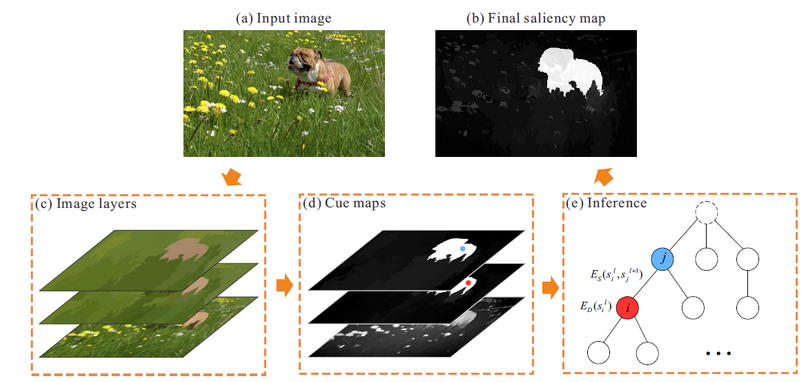
\includegraphics[width=0.95\textwidth]{fig/Hierarchy_Yan13}
\end{center}
\caption{An overview of the hierarchical framework. Three image layers are extracted from the input, and then  saliency cues from each of these layers are computed. They are finally fed into a hierarchical model to get the final results.}
\label{fig:hier_yan13}
\end{figure}

For the purpose of their research the authors made a new database available to the community, the Complex Scene Saliency dataset (CSSD) and the Extended CSSD (ECSSD), described in Section \ref{subsec:cssd}. The executable of their software is also available from the project link (\cite{ecssd_db}), but not the source code. The authors report better performance of their method on MSRA-1000 and (E)CSSD datasets compared to $11$ other state-of-the-art methods.

\subsection{Salient regions}

For the {\em object/scene identificaiton} task, the main question is whether two images taken at different times or under different viewing, lightig or acquizition conditions depict the same object/scene. One way of answerring this question is to compare sets of local characteristic features, extracted reliably and independantly from the two images.

Detecting automatically {\em salient}, e.g.  interesting, distinct, characteristic and repeatably find-able regions from an image is a major research topic in the area of image {\em feature extraction}. The salient regions are one type of features which can offer useful representation of images along with interest points, edges, ridges etc. Usually the first step is automatically extracting salient regions using an salient/interest region {\em detector} followed by describing each region/patch using a region {\em descriptor}. As a final step, two sets of region descriptors are compared and {\em matched} in order to establish correspondences between the images. The main application areas are wide-baseline stereo matching, panoramas stitching,  and identification of scenes and objects. 

One very important and desired property of such region detection is {\em affine covariance}.  The affine covariance property refers to the requirement that these regions should correspond to the same pre-image for different viewpoints and geometric transformations. In the literature that property is often referred to as {\em affine invariance} to these transformations. 
This concept is shown on figure \ref{fig:affreg}. The figure illustrates that an affine salient regions detector has automatically and independently detected the same pre-image regions on both images. Some detectors provide arbitrarily shaped regions, others detect elliptical regions. For the purpose of comparison, the (equivalent) elliptical regions are usually used and shown.
\begin{figure}[H]
\begin{center}
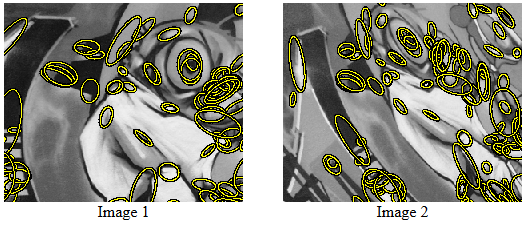
\includegraphics[width=0.95\textwidth]{fig/AffineRegions}
\end{center}
\caption{Example of affine regions detection. Image2 is affinely transformed version of Image1.}
\label{fig:affreg}
\end{figure}

\subsubsection{Detectors}
A decade ago, a seminal paper by the Visual Geometry Group in Oxford, compared the existing affine-covariant region detectors in \cite{Mikolajczyk:2005}. A clear conclusion of this comparative study is the the  {\em  Maximally Stable Extremal Regions (MSER)} detector (\cite{Matas2002BMVC}) is the winner in many of the test scenarios and since then, the MSER detector has become a de-facto standard in the field (for example is now an integral part of the MATLAB Computer Vision System Toolbox). For common implementations of MSER, the reader is referred to \ref{soft:salreg:sec}.

After this comparative study, several researchers have proposed improvements to the MSER detector though none of them increased the performance drastically. 
In \cite{Forssen07} an MSER color extension is proposed. The author calls his detector {\em Maximally stable color region (MSCR)}. In comparison on the well-known Visual Geometry Group in Oxford test image sets (\cite{vgg_soft_data}) with known homographies to the original MSER detector, the simple color MSER extension (MSER3) and a color blob detector, the MSCR performs better in most cases. The executables of the software for MSCR and blob detectors are available at the author's homepage \cite{forssen07_soft}.

The MSER detector has been also extended in 3D to {\em Maximally Stable Volumes (MSVs)} in \cite{DonoserB06}. The MSVs have been used to successfully segment 3D medical images and paper fiber networks.

In \cite{Fan08} a structure-guided salient region detector (SGSR) is introduced. It is based on entropy-based saliency theory and shows competitive performance.

In \cite{Wang14} another enhancement of MSER is proposal, namely with the Canny edge detector. The dilation operator is used on the detected edges to remove ambiguous edges, which makes the interest regions more representative. The improved MSER shows better performance than the original MSER in image classification in the bag of words framework, though original comparison of repeatably (\cite{Mikolajczyk:2005}) is not presented. 

In the context of humpback whale identification, Ranguelova et al. \cite{RangMSSR06, RangHumpb06} have proposed {\em Morphology based Stable Salient Regions (MSSR) } detector which is not better than MSER on repeatably, but mostly on less number of regions (which is important in the matching step) and salient perception. Within the eStep, NLeSc's technology platform, some research is ongoing to improve MSSR. The related code is available in the (for now private) \href{https://github.com/NLeSC/LargeScaleImaging/tree/master/Software}{git NLeSc repository}.

\subsubsection{Descriptors}
Another important performance evaluation paper from the Oxford Vision group has compared the salient region descriptors \cite{MS05}. The conclusion of the performance evaluaiton was the the {\em Gradient location-orientation histogram (GLOH)} detector was performing best (recall and precision) followed closely by the {\em Scale Invariant Feature Transform (SIFT)} descriptor \cite{Lowe:2004}. The SIFT descriptor has been the most popular and widely used descriptor in CV for over a decade. 

The idea behind SIFT Transform is finding the extrema in scale-space. These extrema found from all possible scales and image locations are the potential iterest points (another important class of features forimage description andmatching). Then only the most stable points are selected. One or more orientations are assigned to a point based onthe local gradient directions, while invariance to reansformations is achived by computing these orientaitons from all possible transformed versions of the data.  This histogram of (usually $128$) orientaitons are the keypoint descriptor. For applying SIFT descriptor on salient regions, only the descriptor steps are performed. 
There are many variants of the SIFT descriptor, all based on floating point aritmetic, for example, SURF\cite{Bay:2008:SURF} and also GLOH \cite{MS05}, designed to improve distinctiveness.

There is an important class of descriptors which offer computationally more tractable solution to region/patch description, the {\em binary descriptors}. Examples of such descriptors are  {\em FAST} \cite{Rosten:2006}, {\em Binary robust independant elementary features (BRIEF)}\cite{Calonder:2010}, {\em Binary Robust Invariant Keypoints (BRISK)} \cite{Leutenegger:2011}, {\em  ORB} \cite{Rublee:2011}, etc.

Another more recent performance paper compares their performance also in comparision to the established descriptors like SIFT or SURF \cite{conf/icpr/MiksikM12}.
{\bf TO DO- main conclusions paper}.

More recently simpler to compute, but also very rich and distinctive descriptors have been proposed. An important class is the so called binary descriptors. For example, the {\em Binary Online Learned Descriptor (BOLD)}, \cite{Balntas_2015_CVPR}.....

\subsubsection{Matching}

\subsection{Convolutional Neural Networks}

Recently, an interesting article which compares the matching of salient regions  with CNNs with matching with SIFT descriptor have been published \cite{FischerDB14}. The authors have also recorded a new larger dataset, compared to the only $48$ images in the comparative study paper, covering larger class of image transformations with more images (see \ref{sec:salregdb}). The goal of the paper is to study the regions/patches descriptors, not to evaluate detectors. For the detection step, the standard MSER detector have been used. The paper concludes that the CNN trained features are consistently better than the SIFT descriptor, for the price of a higher computational cost.